\graphicspath{{img/}}

\subsection{Decodificación manual}

Se codifican palabras recibidas propuestas siguiendo el algoritmo de cuatro casos. Se hace el desarrollo en hoja cálculo adjunta en repositorio (\href{https://github.com/AbelCorvalan0/fec-lab2/tree/main/reference-calc}{\textbf{reference.ods}}). En la siguiente figura se presentan los casos de obtención de la máscara de error:

%% Llevar al archivo LaTeX local
\begin{figure}[h!]
    \centering
    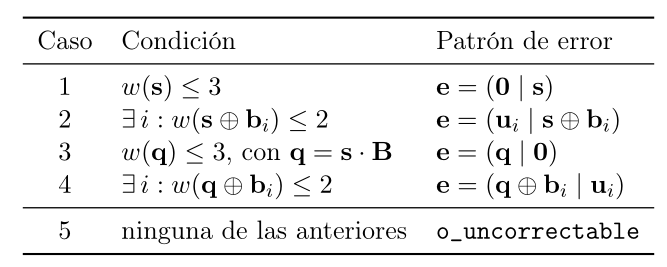
\includegraphics[width=0.5\linewidth]{correction-cases.png}
    \caption{Casos de evaluación para correción}
    \label{fig:correction cases}
\end{figure}

Las palabras recibidas propuestas para evaluar en el codificador son las siguientes:

\begin{table}[h!]
    \centering
    \begin{tabular}{ccc}
        \hline
        $r_1$ & $r_2$ & $r_3$ \\
        \hline
        \texttt{0xA5D9A6} & \texttt{0xA5F9A4} & \texttt{0xA5C9AA} \\
        \hline
    \end{tabular}
\end{table}

Se calculan los vectores $s$ y $q$. Estos vectores se obtienen realizando las siguientes operaciones:

$$ \boxed{s = r[23:12]  \cdot \textbf{B} \, \oplus r[11:0]} $$

$$ q = s \cdot \textbf{B} = (r[23:12]  \cdot \textbf{B} \, \oplus r[11:0]) \cdot \textbf{B} $$

$$ \boxed{q = r[23:12] \oplus (r[11:0] \cdot \textbf{B})} $$

A continuación se muestra la matriz $\textbf{B}$:

\[
\textbf{B} =
\left[
\begin{array}{@{}cccccccccccc@{}}
1&0&0&1&1&0&0&0&1&1&1&1\\
0&1&0&0&1&1&1&0&0&1&1&1\\
0&0&1&1&0&1&0&1&0&1&1&1\\
1&0&1&1&1&1&1&0&0&0&1&0\\
1&1&0&1&1&1&0&1&0&0&0&1\\
0&1&1&1&1&1&0&0&1&1&0&0\\
0&1&0&1&0&0&1&1&1&1&0&1\\
0&0&1&0&1&0&1&1&1&1&1&0\\
1&0&0&0&0&1&1&1&1&0&1&1\\
1&1&1&0&0&1&1&1&0&1&0&0\\
1&1&1&1&0&0&0&1&1&0&1&0\\
1&1&1&0&1&0&1&0&1&0&0&1
\end{array}
\right]
\]

Se obtienen los siguientes conjuntos de vectores $s$ y $q$ para las palabras a decodificar:

\begin{table}[h!]
    \centering
    \begin{tabular}{ccc}
        \hline
        $r$ & $s$ & $q$ \\
        \hline
        \texttt{0xA5D9A6} & \texttt{0xEAA} & \texttt{0xEAA} \\
        \texttt{0xA5F9A4} & \texttt{0x1B2} & \texttt{0xEAA} \\
        \texttt{0xA5C9AA} & \texttt{0x00F} & \texttt{0x7BC} \\
        \hline
    \end{tabular}
\end{table}

Estos resultados y los cálculos que siguen, se realizaron en la hoja de cálculo mencionada anteriormente (\href{https://github.com/AbelCorvalan0/fec-lab2/tree/main/reference-calc}{\textbf{reference.ods}}).

%%%%%%%%%%%%%%%%%%%%%%%%%%%%%%%%%%%%%%%%%%%%%
% r1 = 0xA5F9A6
%%%%%%%%%%%%%%%%%%%%%%%%%%%%%%%%%%%%%%%%%%%%%

\subsection{Palabra recibida 1: $0xA5D9A6$}

\subsubsection{Caso 1}

Luego se evalúa el peso del vector $s$ y la condición correspondiente al primer caso:

$$ weight(s) \leq 3 = 7 \leq 3 = FALSE $$

Por lo que no se cumple con la primera condición.

\subsubsection{Caso 2}

Se evalúa si algún peso de las operaciones $s \oplus b_{i}$ es menor a 2. Esto es:

$$ weight(S \oplus b_{i}) \leq 2 $$

\begin{table}[h!]
    \centering
    \begin{tabular}{lc}
        \hline
        \textbf{Expresión} & \textbf{Peso} \\
        \hline
        $\operatorname{weight}(S \oplus b_0)$  & 6  \\
        $\operatorname{weight}(S \oplus b_1)$  & 6  \\
        $\operatorname{weight}(S \oplus b_2)$  & 10 \\
        $\operatorname{weight}(S \oplus b_3)$  & 4  \\
        $\operatorname{weight}(S \oplus b_4)$  & 8  \\
        $\operatorname{weight}(S \oplus b_5)$  & 6  \\
        $\operatorname{weight}(S \oplus b_6)$  & 8  \\
        $\operatorname{weight}(S \oplus b_7)$  & 4  \\
        $\operatorname{weight}(S \oplus b_8)$  & 6  \\
        $\operatorname{weight}(S \oplus b_9)$  & 6  \\
        $\operatorname{weight}(S \oplus b_{10})$ & 4 \\
        $\operatorname{weight}(S \oplus b_{11})$ & 2 \\
        \hline
    \end{tabular}
\end{table}

Entonces se tiene que la operación que cumple con la condición es:

$$ weight(S \oplus b_{11}) = 2 \leq 2$$

Entonces la máscara de error se construye de la siguiente forma:

$$ \textbf{e} = (u_{i} | (s \oplus bi)) $$

En este caso resulta:

$$ \boxed{\textbf{e} = 0x000001}$$

%%%%%%%%%%%%%%%%%%%%%%%%%%%%%%%%%%%%%%%%%%%%%
% r2 = 0xA5F9A4
%%%%%%%%%%%%%%%%%%%%%%%%%%%%%%%%%%%%%%%%%%%%%
\subsection{Palabra recibida 2: $0xA5F9A4$}

\subsubsection{Caso 1}

Luego se evalúa el peso del vector $s$ y la condición correspondiente al primer caso:

$$ weight(s) \leq 3 = 5 \leq 3 = FALSE $$

Por lo que no se cumple con la primera condición.

\subsubsection{Caso 2}

Se evalúa si algún peso de las operaciones $s \oplus b_{i}$ es menor a 2. Esto es:

$$ weight(S \oplus b_{i}) \leq 2 $$

\begin{table}[h!]
    \centering
    \begin{tabular}{lc}
        \hline
        \textbf{Expresión} & \textbf{Peso} \\
        \hline
        $\operatorname{weight}(S \oplus b_0)$  & 6  \\
        $\operatorname{weight}(S \oplus b_1)$  & 6  \\
        $\operatorname{weight}(S \oplus b_2)$  & 6  \\
        $\operatorname{weight}(S \oplus b_3)$  & 4  \\
        $\operatorname{weight}(S \oplus b_4)$  & 6  \\
        $\operatorname{weight}(S \oplus b_5)$  & 8  \\
        $\operatorname{weight}(S \oplus b_6)$  & 6  \\
        $\operatorname{weight}(S \oplus b_7)$  & 4  \\
        $\operatorname{weight}(S \oplus b_8)$  & 6  \\
        $\operatorname{weight}(S \oplus b_9)$  & 8  \\
        $\operatorname{weight}(S \oplus b_{10})$ & 6 \\
        $\operatorname{weight}(S \oplus b_{11})$ & 8 \\
        \hline
    \end{tabular}
\end{table}

Ninguna de las operaciones cumple con la condición.

\subsubsection{Caso 3}

Se calcula el peso del vector $q$. Se tiene:

$$ weight(q) = 7 $$

$$ weight(q) \leq 3 = 7 \leq 3 = FALSE $$

Por lo que no se cumple la condición.

\subsubsection{Caso 4}

Se evalúa si algún peso de las operaciones $q \oplus b_{i}$ es menor a 2. Esto es:

$$ weight(q \oplus b_{i}) \leq 2 $$

\begin{table}[h!]
    \centering
    \begin{tabular}{lc}
        \hline
        \textbf{Expresión} & \textbf{Peso} \\
        \hline
        $\operatorname{weight}(q \oplus b_0)$  & 6  \\
        $\operatorname{weight}(q \oplus b_1)$  & 6  \\
        $\operatorname{weight}(q \oplus b_2)$  & 10 \\
        $\operatorname{weight}(q \oplus b_3)$  & 4  \\
        $\operatorname{weight}(q \oplus b_4)$  & 8  \\
        $\operatorname{weight}(q \oplus b_5)$  & 6  \\
        $\operatorname{weight}(q \oplus b_6)$  & 8  \\
        $\operatorname{weight}(q \oplus b_7)$  & 4  \\
        $\operatorname{weight}(q \oplus b_8)$  & 6  \\
        $\operatorname{weight}(q \oplus b_9)$  & 6  \\
        $\operatorname{weight}(q \oplus b_{10})$ & 4 \\
        $\operatorname{weight}(q \oplus b_{11})$ & 2 \\
        \hline
    \end{tabular}
\end{table}

Entonces se tiene que la operación que cumple con la condición es:

$$ weight(q \oplus b_{11}) = 2 \leq 2$$

Entonces la máscara de error se construye de la siguiente forma:

$$ \textbf{e} = ((q \oplus bi) | u_{i}) $$

En este caso resulta:

$$ \boxed{\textbf{e} = 0x003001}$$

%%%%%%%%%%%%%%%%%%%%%%%%%%%%%%%%%%%%%%%%%%%%%
% r3 = 0xA5C9AA
%%%%%%%%%%%%%%%%%%%%%%%%%%%%%%%%%%%%%%%%%%%%%
\subsection{Palabra recibida 3: $0xA5C9AA$}

\subsubsection{Caso 1}

Se evalúa el peso del vector $s$ y la condición correspondiente al primer caso:

$$ weight(s) \leq 3 = 4 \leq 3 = FALSE $$

Por lo que no se cumple con la primera condición.

\subsubsection{Caso 2}

Se evalúa si algún peso de las operaciones $s \oplus b_{i}$ es menor a 2. Esto es:

$$ weight(S \oplus b_{i}) \leq 2 $$

\begin{table}[h!]
    \centering
    \begin{tabular}{lc}
        \hline
        \textbf{Expresión} & \textbf{Peso} \\
        \hline
        $\operatorname{weight}(S \oplus b_0)$    & 3 \\
        $\operatorname{weight}(S \oplus b_1)$    & 5 \\
        $\operatorname{weight}(S \oplus b_2)$    & 5 \\
        $\operatorname{weight}(S \oplus b_3)$    & 9 \\
        $\operatorname{weight}(S \oplus b_4)$    & 9 \\
        $\operatorname{weight}(S \oplus b_5)$    & 7 \\
        $\operatorname{weight}(S \oplus b_6)$    & 5 \\
        $\operatorname{weight}(S \oplus b_7)$    & 5 \\
        $\operatorname{weight}(S \oplus b_8)$    & 5 \\
        $\operatorname{weight}(S \oplus b_9)$    & 9 \\
        $\operatorname{weight}(S \oplus b_{10})$ & 7 \\
        $\operatorname{weight}(S \oplus b_{11})$ & 7 \\
        \hline
    \end{tabular}
\end{table}

Ninguna de las operaciones cumple con la condición.

\subsubsection{Caso 3}

Se calcula el peso del vector $q$. Se tiene:

$$ weight(q) = 8 $$

$$ weight(q) \leq 3 = 8 \leq 3 = FALSE $$

Por lo que no se cumple la condición.

\subsubsection{Caso 4}

Se evalúa si algún peso de las operaciones $q \oplus b_{i}$ es menor a 2. Esto es:

$$ weight(q \oplus b_{i}) \leq 2 $$

\begin{table}[h!]
    \centering
    \begin{tabular}{lc}
        \hline
        \textbf{Expresión} & \textbf{Peso} \\
        \hline
        $\operatorname{weight}(q \oplus b_0)$    & 7 \\
        $\operatorname{weight}(q \oplus b_1)$    & 7 \\
        $\operatorname{weight}(q \oplus b_2)$    & 7 \\
        $\operatorname{weight}(q \oplus b_3)$    & 7 \\
        $\operatorname{weight}(q \oplus b_4)$    & 7 \\
        $\operatorname{weight}(q \oplus b_5)$    & 3 \\
        $\operatorname{weight}(q \oplus b_6)$    & 3 \\
        $\operatorname{weight}(q \oplus b_7)$    & 3 \\
        $\operatorname{weight}(q \oplus b_8)$    & 9 \\
        $\operatorname{weight}(q \oplus b_9)$    & 5 \\
        $\operatorname{weight}(q \oplus b_{10})$ & 5 \\
        $\operatorname{weight}(q \oplus b_{11})$ & 5 \\
        \hline
    \end{tabular}
\end{table}

Se tiene que ninguna de las operaciones cumple con la condición.

De esta forma hace que la palabra recibida sea clasificada como incorregible:

$$ \boxed{\textbf{e} = 0x000000} $$